\newpage
\section{Aufbau und Durchführung}
\label{sec:Durchführung}
\subsection{Aufbau}
\begin{figure}
 \centering
 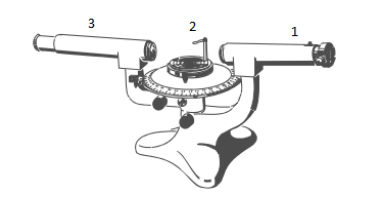
\includegraphics[width=0.7\textwidth]{Aufbau.png}
 \caption{Darstellung des Spektralapparates.\cite{sample}}
 \label{fig:apparat}
 \end{figure}
In Abbildung \ref{fig:apparat} ist ein Spektralapparat zu sehen, dieser besteht wesentlich aus dem Kollimatorrohr mit Spaltblende (Position 1), dies bündelt und parallelisiert die eingehende Strahlung.
Am Gitter (Position 2) wird die Strahlung gebeugt und im Fernrohr (Position 3) kann das Spektrum beobachtet werden. Das Fernrohr ist beweglich gelagert, sodass die unterschiedlichen Maxima
beobachten werden können und die zugehörigen Beugungswinkel an der Teilkreisplatte abgelesen werden können. Im Fernrohr befindet sich auch ein Okularmikrometer, damit lässt sich der Abstand
zweier Spektrallinien abmessen.
Eine Lichtquelle kann noch vor die Spaltblende des Kollimatorrohrs plaziert werden.

\subsection{Eichung mittels Heliumspektrum}
Zur Eichung des Okularmikrometers wird das Heliumspektrum verwendet. Zunächst werden die Beugungswinkel der verschiedenen Spektrallinien bestimmt.
Weiterhin wird das Fernrohr so justiert, dass zwei benachbarte Spektrallinien mit bekannter Wellenlänge auf dem Okularmikrometer zu sehen sind, deren Abstand wird dann bestimmt.
Dies geschieht für mehrere benachbarte Spektrallinienpaare.

\subsection{Vermessung der Dublettlinien von Alkalimetallen}
Die Helium-Lichtquelle wird durch verschiedene Lichtquellen von Alkalimetallen ausgetauscht.
Die Position der Dublettlinien wird mittels Messung der Beugungswinkel bestimmt und
anschließend die Abstände verschiedener Dublettlinien werden mit dem Okularmikrometer vermessen.
